In this final chapter we present the signal reconstruction efficiencies for the considered
 Hidden Valley
model depending on the masses and lifetimes of the exotic \Higgs and \X particles. 
We then unblind the data in the signal region and confront it with a
 signal hypothesis. The data is consistent with the background only hypothesis, therefore we
compute upper limits depending on the reconstruction efficiency of the signal models.

\section{Long-lived particles reconstruction efficiency}
\label{sec:signalefficiency}

In order to visualize the capabilities of the CMS detector for reconstructing long-lived particles decaying to 
dijets, 
the reconstructed dijet mass and $L_{xy}$ distributions for selected signal models are shown in Figure
\ref{fig:signal}. We assume the cross-section of the $\Higgs \to 2\X$ process to be 1 pb and the branching 
ratio to quarks ($\X \to \qq$) to be 100\%.

\begin{figure}[htbp]
\centering
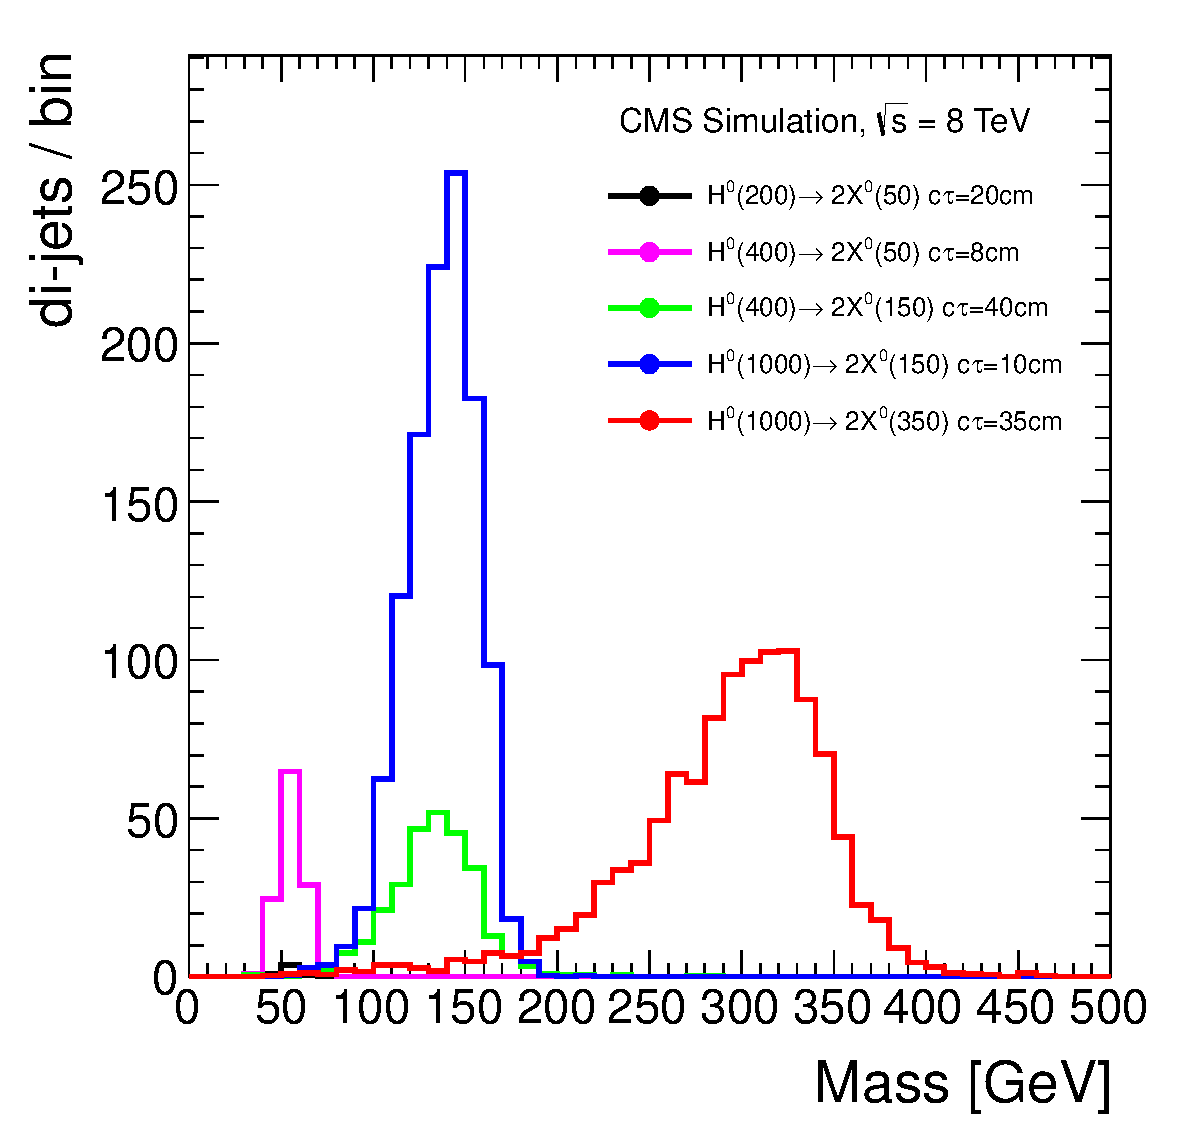
\includegraphics[width=0.49\textwidth]{plots/signal/mass.pdf}
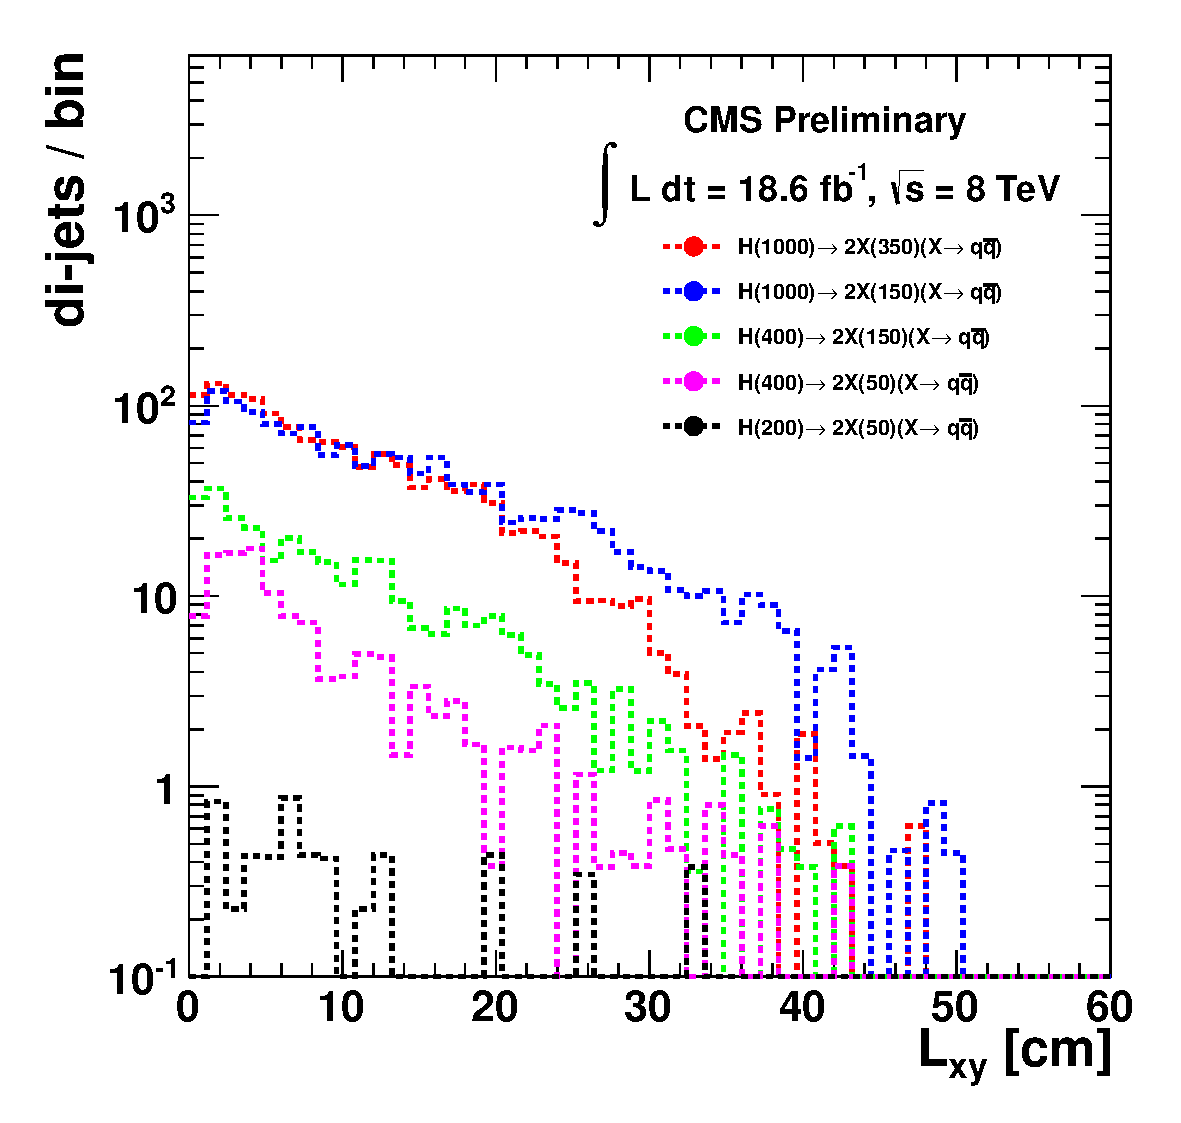
\includegraphics[width=0.49\textwidth]{plots/signal/Lxy.pdf}
\caption{The reconstructed dijet mass and $L_{xy}$ for selected signal models; central lifetime out of the three available is presented.\label{fig:signal}}
\end{figure}

The signal reconstruction efficiency is obtained by applying the final selection
criteria (Section \ref{sec:cutvalues}) to the dijet candidate that have been chosen 
after candidate preselection and counting the surviving events.
The efficiency for all considered signal models 
is presented in Table 
\ref{tab:sigeff}. 

\begin{table}[htbp]
\caption{
Signal reconstruction efficiency ($\epsilon$) for $\Higgs \to 2\X \left(\X \to \qq\right)$ 
in simulated signal models.
The trigger and reconstruction efficiencies are both included in the efficiency.
The uncertainties are statistical only.\label{tab:sigeff}}
\centering
\begin{tabular}{llccc}
\hline
$\Higgs$ [GeV] & $\X$ [GeV] & c$\tau$ [cm] & $\langle L_{xy} \rangle$ [cm] & $\epsilon$ [\%] \\
\hline
200 & 50 & 2 & 3 & $0.25 \pm 0.05$ \\
200 & 50 & 20 & 30 & $0.15 \pm 0.04$ \\
\hline
400 & 50 & 0.8 & 2.6 & $5.6 \pm 0.2$ \\
400 & 50 & 8 & 26 &  $3.3 \pm 0.2$ \\
400 & 50 & 80 & 260 & $0.3 \pm 0.06$ \\
\hline
400 & 150 & 4 & 3 & $15.6 \pm 0.4$ \\
400 & 150 & 40 & 30 & $7.6 \pm 0.3$ \\
400 & 150 & 400 & 300 & $0.6 \pm 0.1$ \\
\hline
1000 & 150 & 1 & 2.5 & $41.3 \pm 0.5$ \\
1000 & 150 & 10 & 25 & $31.1 \pm 0.5$ \\
1000 & 150 & 100 & 250 & $4.8 \pm 0.2$ \\
\hline
1000 & 350 & 3.5 & 2.9 & $49.2 \pm 0.5$ \\
1000 & 350 & 35 & 29 & $30.9 \pm 0.5$ \\
1000 & 350 & 350 & 290 & $4.4 \pm 0.2$ \\
\hline

\end{tabular}
\end{table}

The signal reconstruction efficiency is examined further as a function of the various
properties of the signal event. 
Figure \ref{fig:effLxy} presents the efficiency as a function of the \X particles
transverse displacement, Figure \ref{fig:effIP2d} shows the efficiency as a function of
the transverse impact parameters of the $\qq$ system, while Figure \ref{fig:effPt} presents
the efficiency as a function of \Higgs and \X particles transverse momenta.

\begin{figure}[htbp]
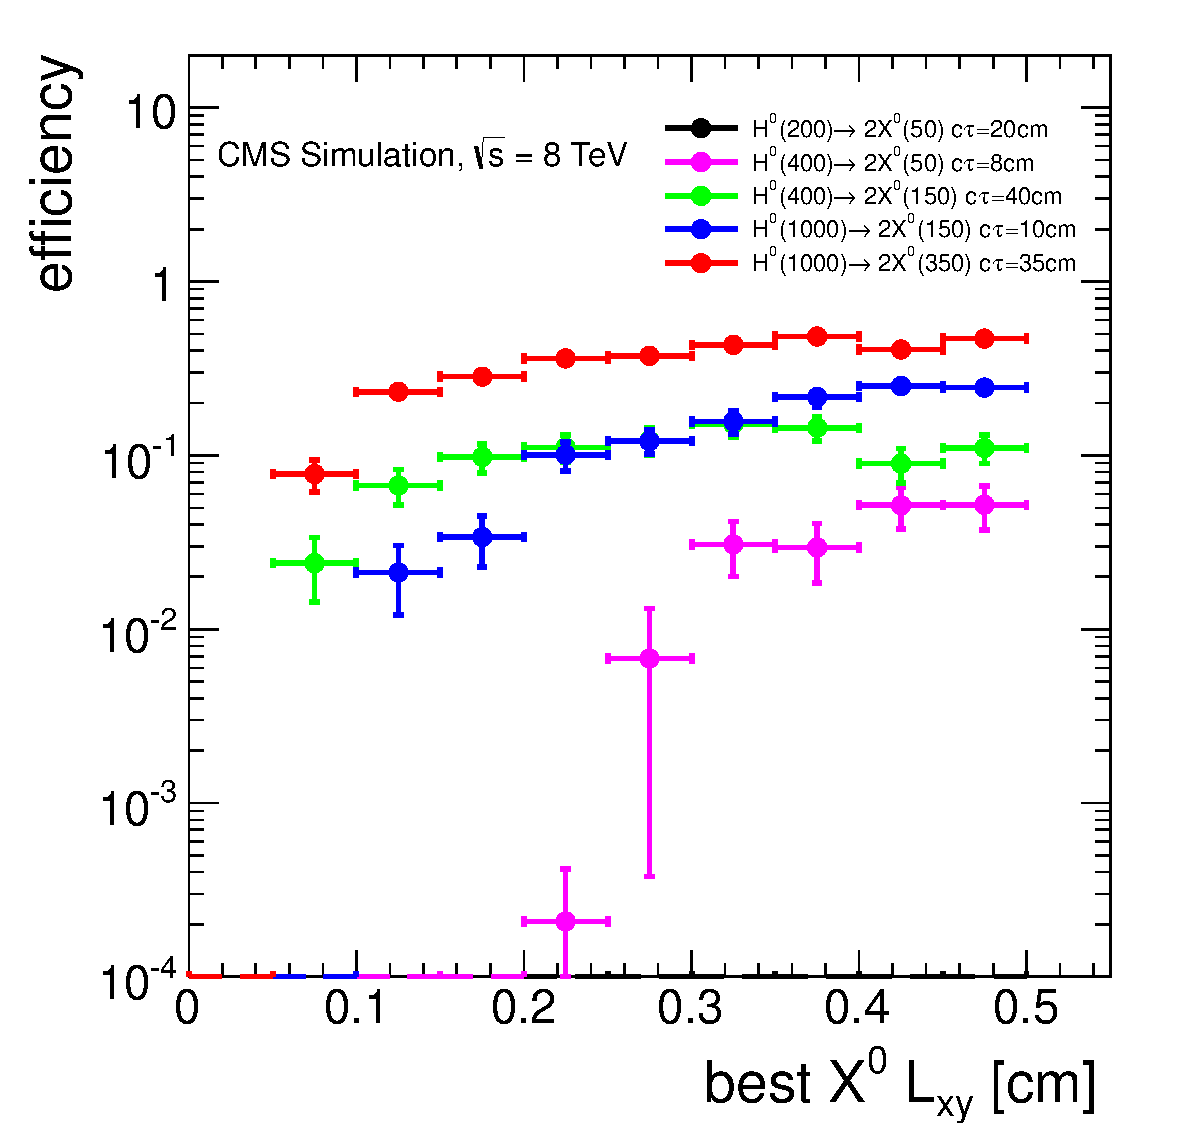
\includegraphics[width=0.49\textwidth]{plots/signal/effSmallLxy.pdf}
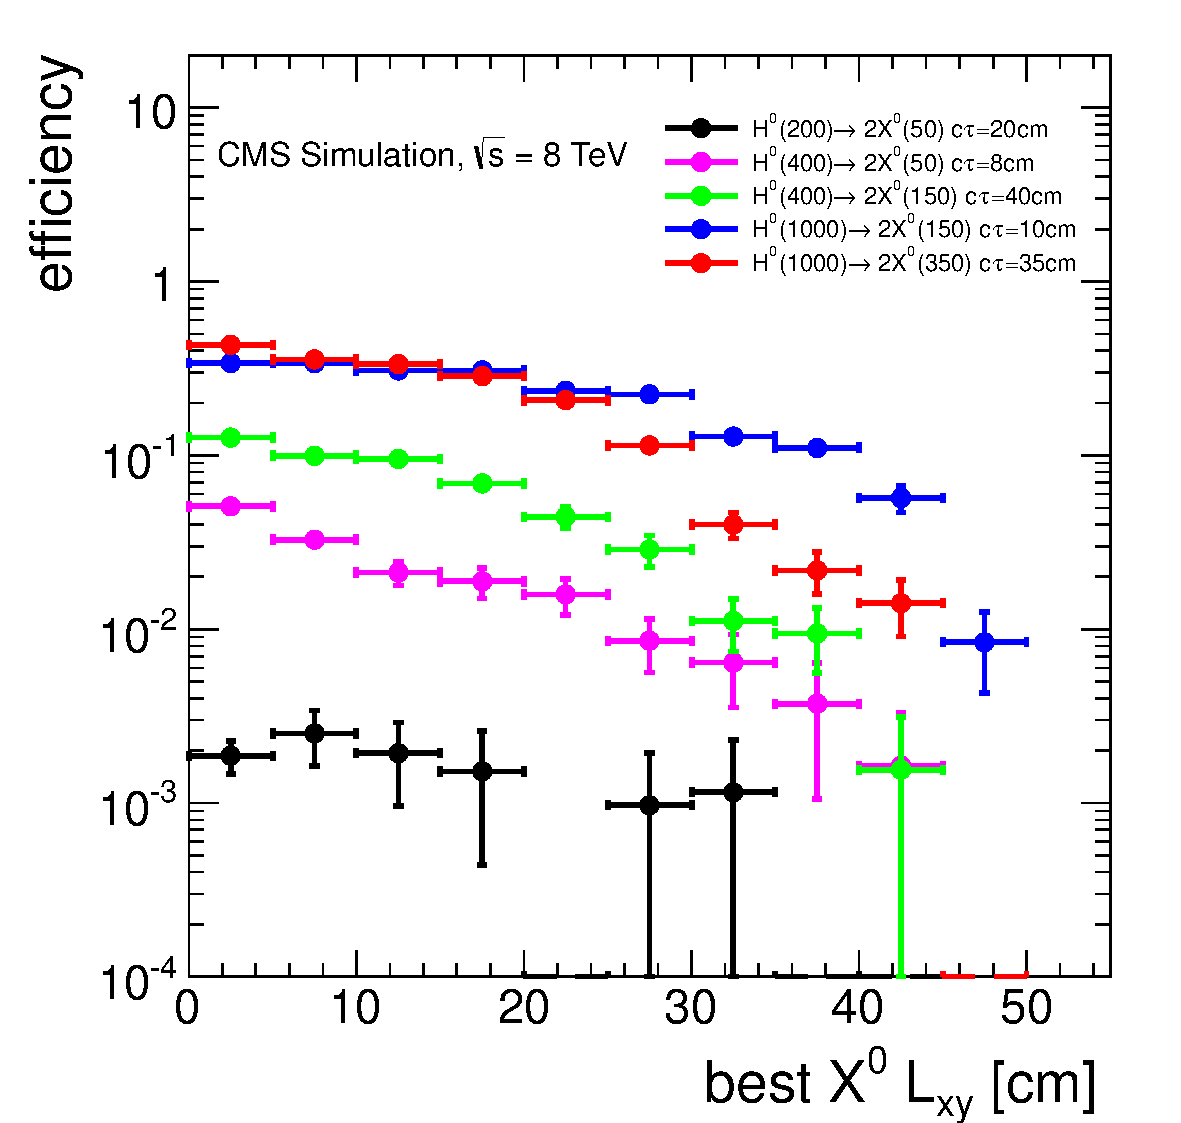
\includegraphics[width=0.49\textwidth]{plots/signal/effLxy.pdf}
\caption{Signal reconstruction efficiency as a function of the \X particle transverse 
displacement ($L_{xy}$). The turn-on curve for small displacement is shown on the left,
while the turn-off for large displacements is presented on the right.\label{fig:effLxy}}
\end{figure}
\begin{figure}[htbp]
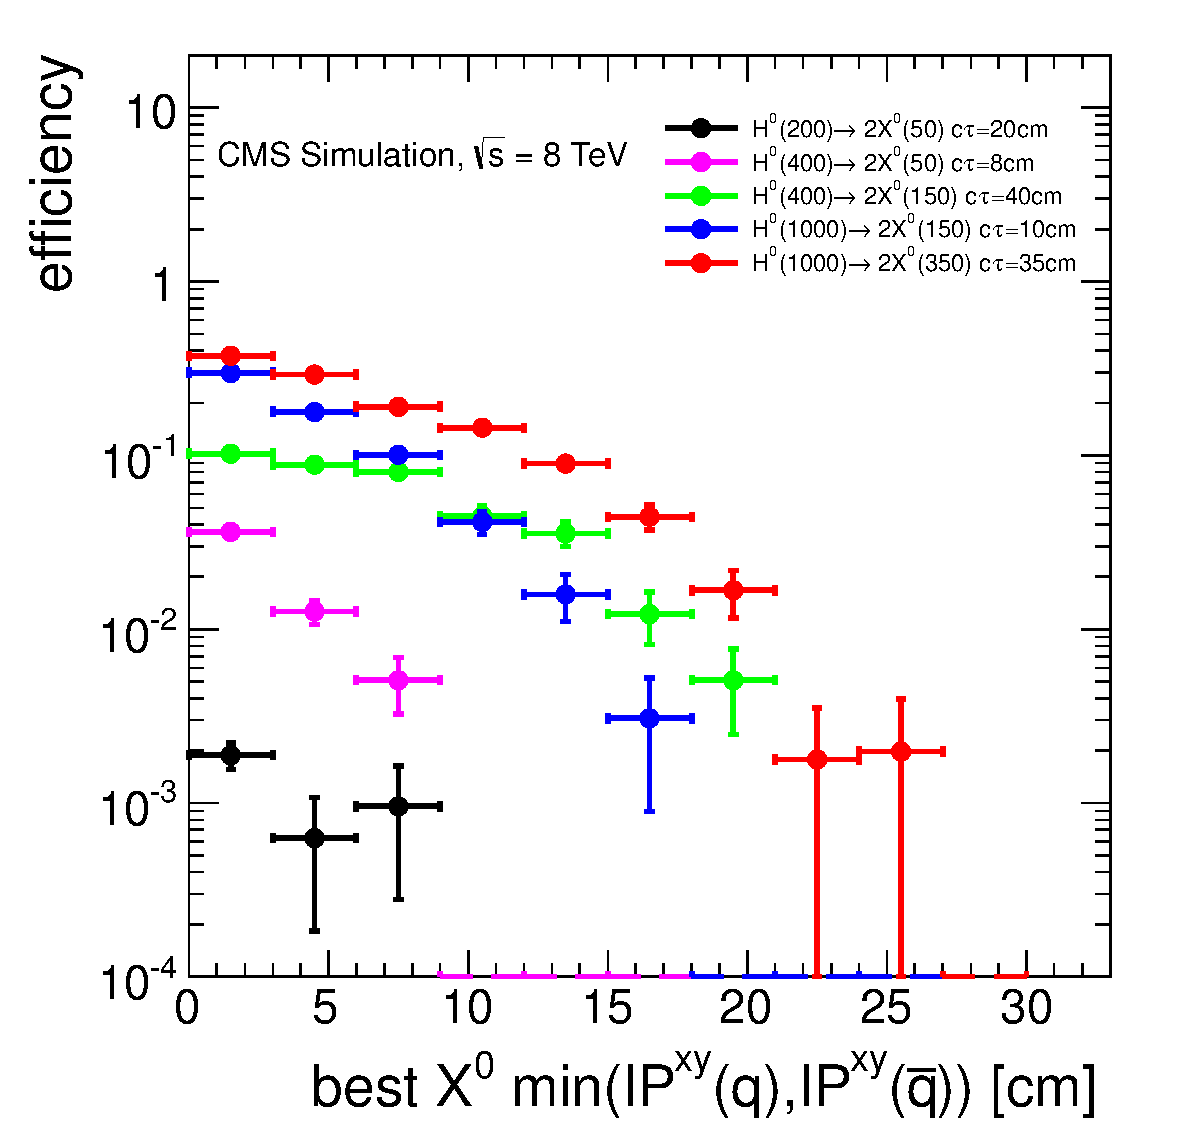
\includegraphics[width=0.49\textwidth]{plots/signal/effIP2dMin.pdf}
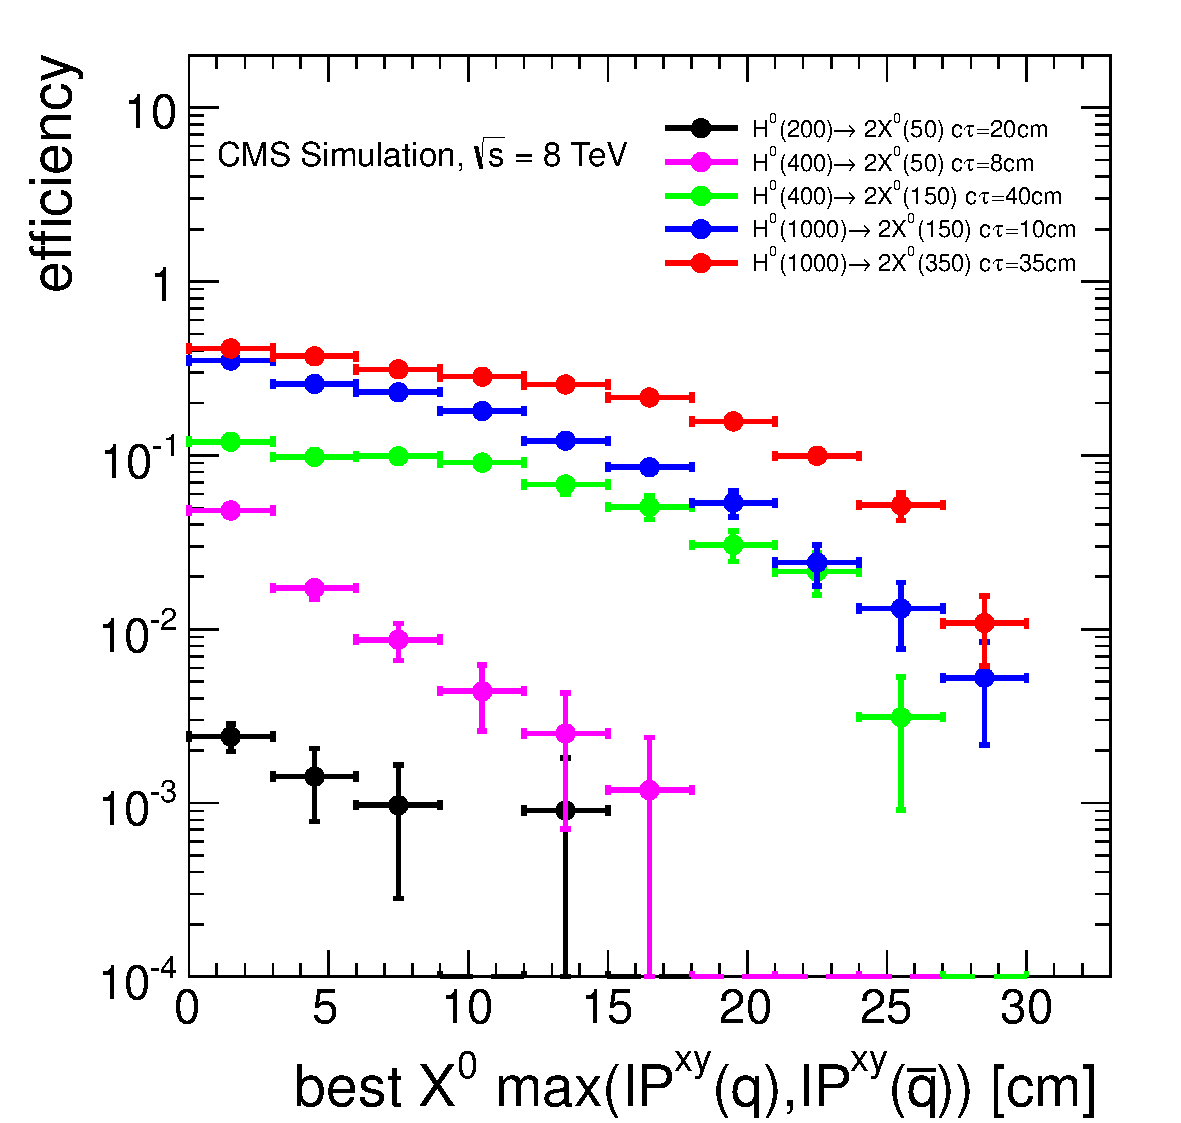
\includegraphics[width=0.49\textwidth]{plots/signal/effIP2dMax.pdf}
\caption{Signal reconstruction efficiency as a function of the transverse impact
parameters of the $\qq$ system. The efficiency as a function of the smaller 
of the two $\qq$ transverse impact parameters
is shown on the left, while the efficiency as a function of the larger one 
is presented on the right.
\label{fig:effIP2d}}
\end{figure}

\begin{figure}[htbp]
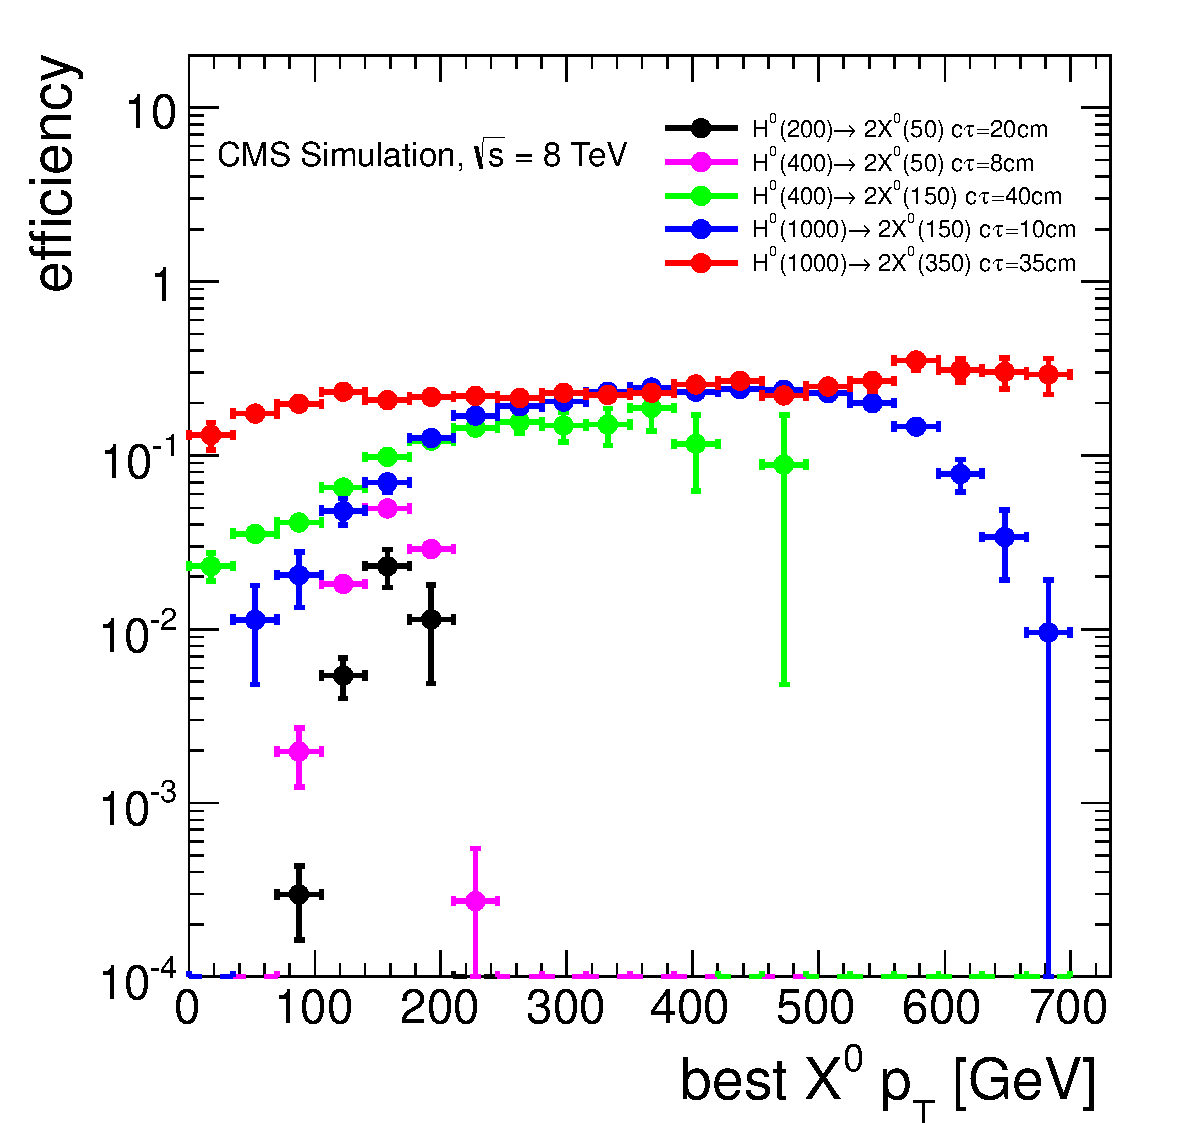
\includegraphics[width=0.49\textwidth]{plots/signal/effXPt.pdf}
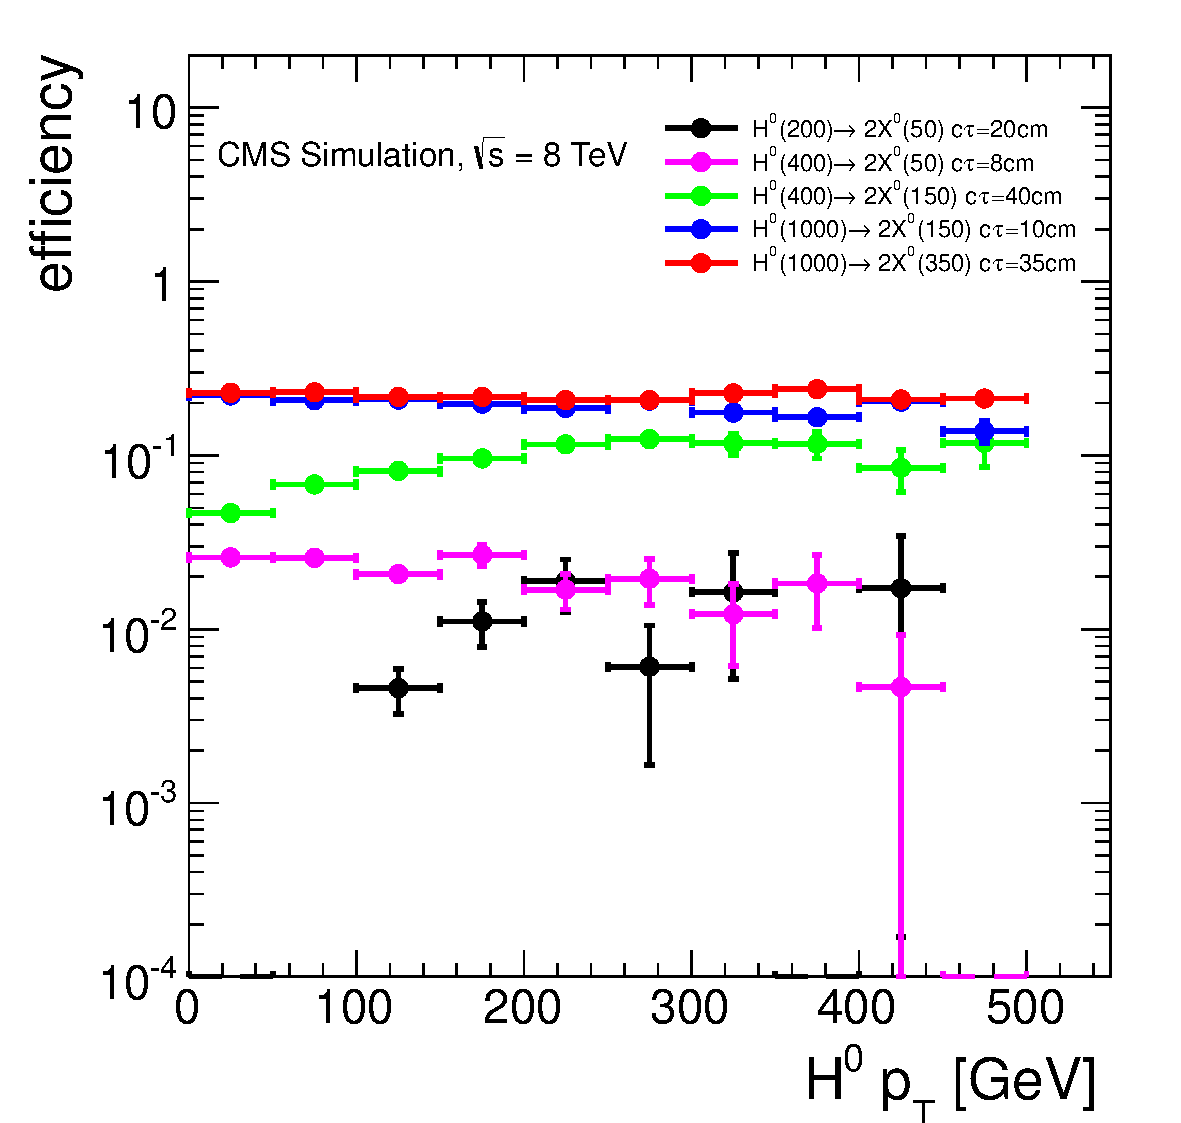
\includegraphics[width=0.49\textwidth]{plots/signal/effHPt.pdf}
\caption{Signal reconstruction efficiency as a function of the \X particle transverse 
momentum (left) and as a function of the \Higgs particle transverse momentum (right).
\label{fig:effPt}}
\end{figure}


\section{Data in the signal region}
\label{sec:fullunblinding}

Table \ref{tab:fullunblinding} summarizes the observed event counts in the signal region for the optimized 
selections detailed in Section \ref{sec:cutvalues}. Data is found in good agreement with the 
background only hypothesis. In addition, the two selected events are examined using event displays
and are found consistent with background events as described in the caption of 
Figure \ref{fig:eventDisplays}.  

\begin{table}[htbp]
\centering
\begin{tabular}{|l|c|c|}
\hline
$\bf L_{xy}$ \bf selection & \bf low & \bf high \\
\hline
\bf Predicted Background & $ 1.60\pm0.58(stat+sys)$ & $ 1.14\pm0.54(stat+sys)$ \\
\hline
\bf Observed events & 2 & 1 \\ 
\hline
\end{tabular}
\caption{Observed events and predicted background for the optimized selections.\label{tab:fullunblinding}}
\end{table}

\begin{figure}
\centering
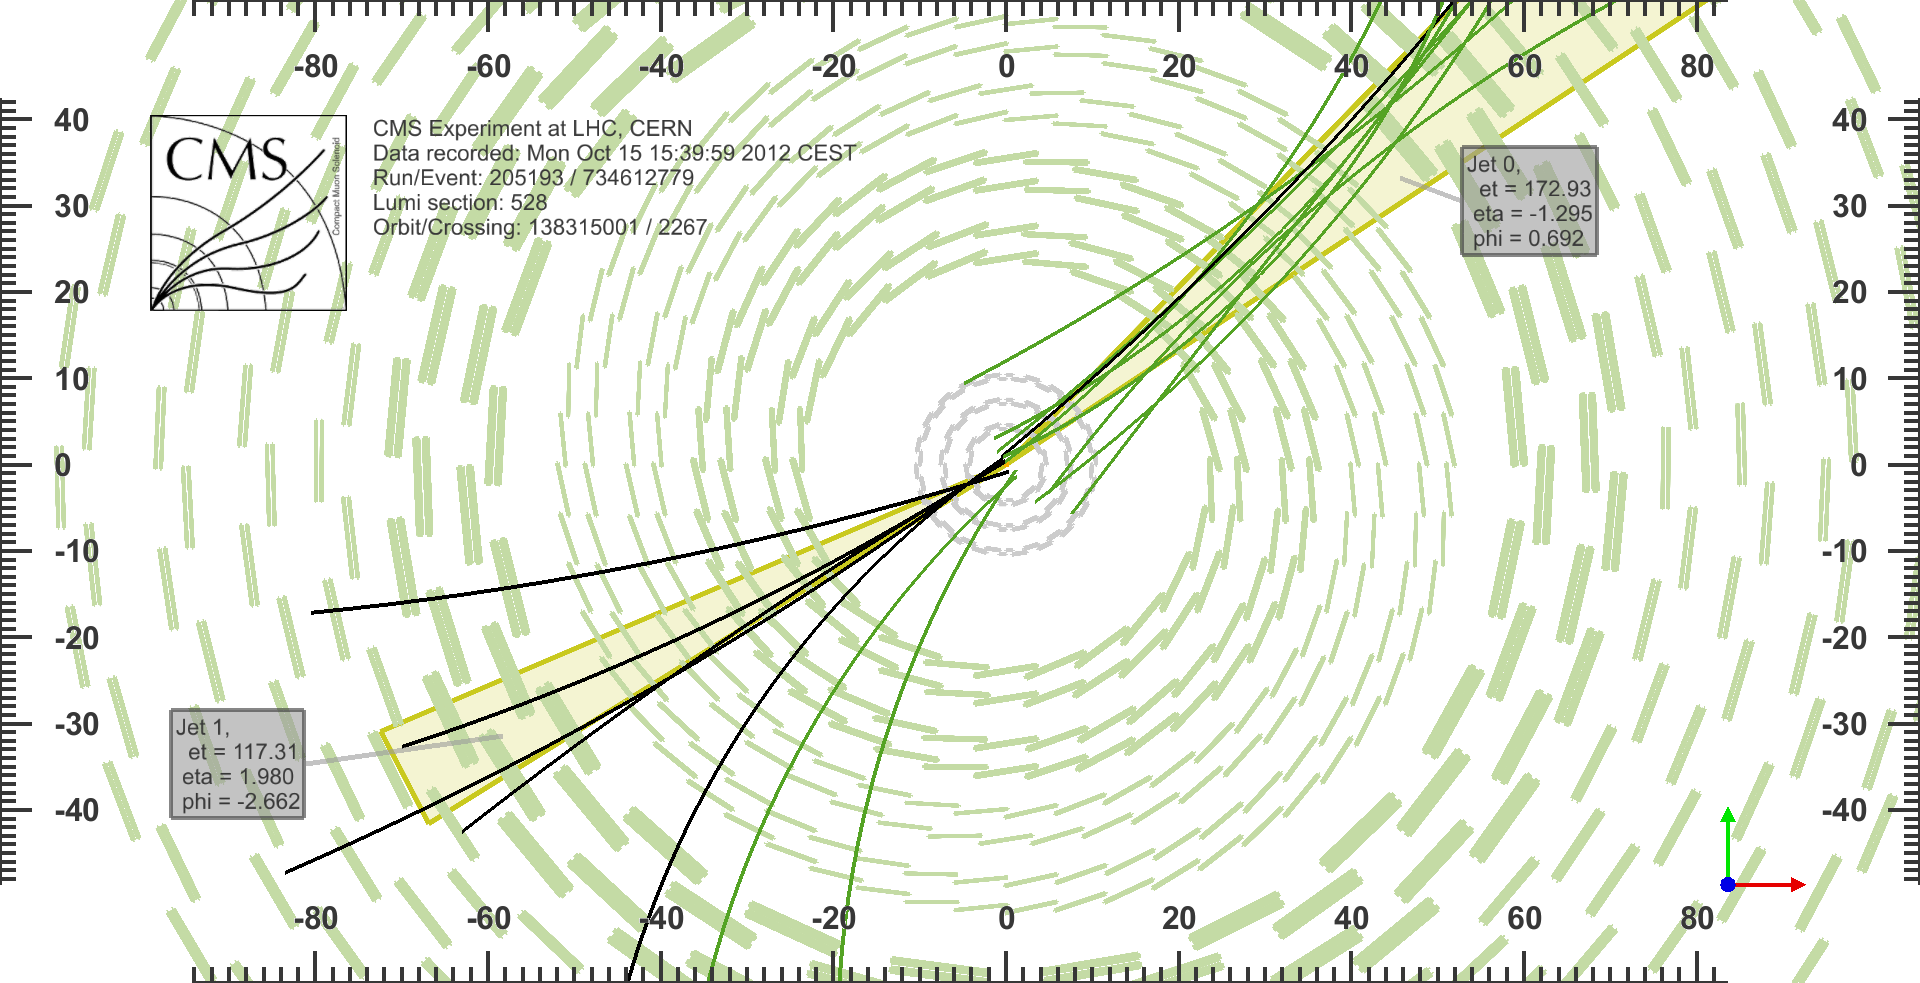
\includegraphics[width=0.9\textwidth]{plots/displays/candidate1_display.png}
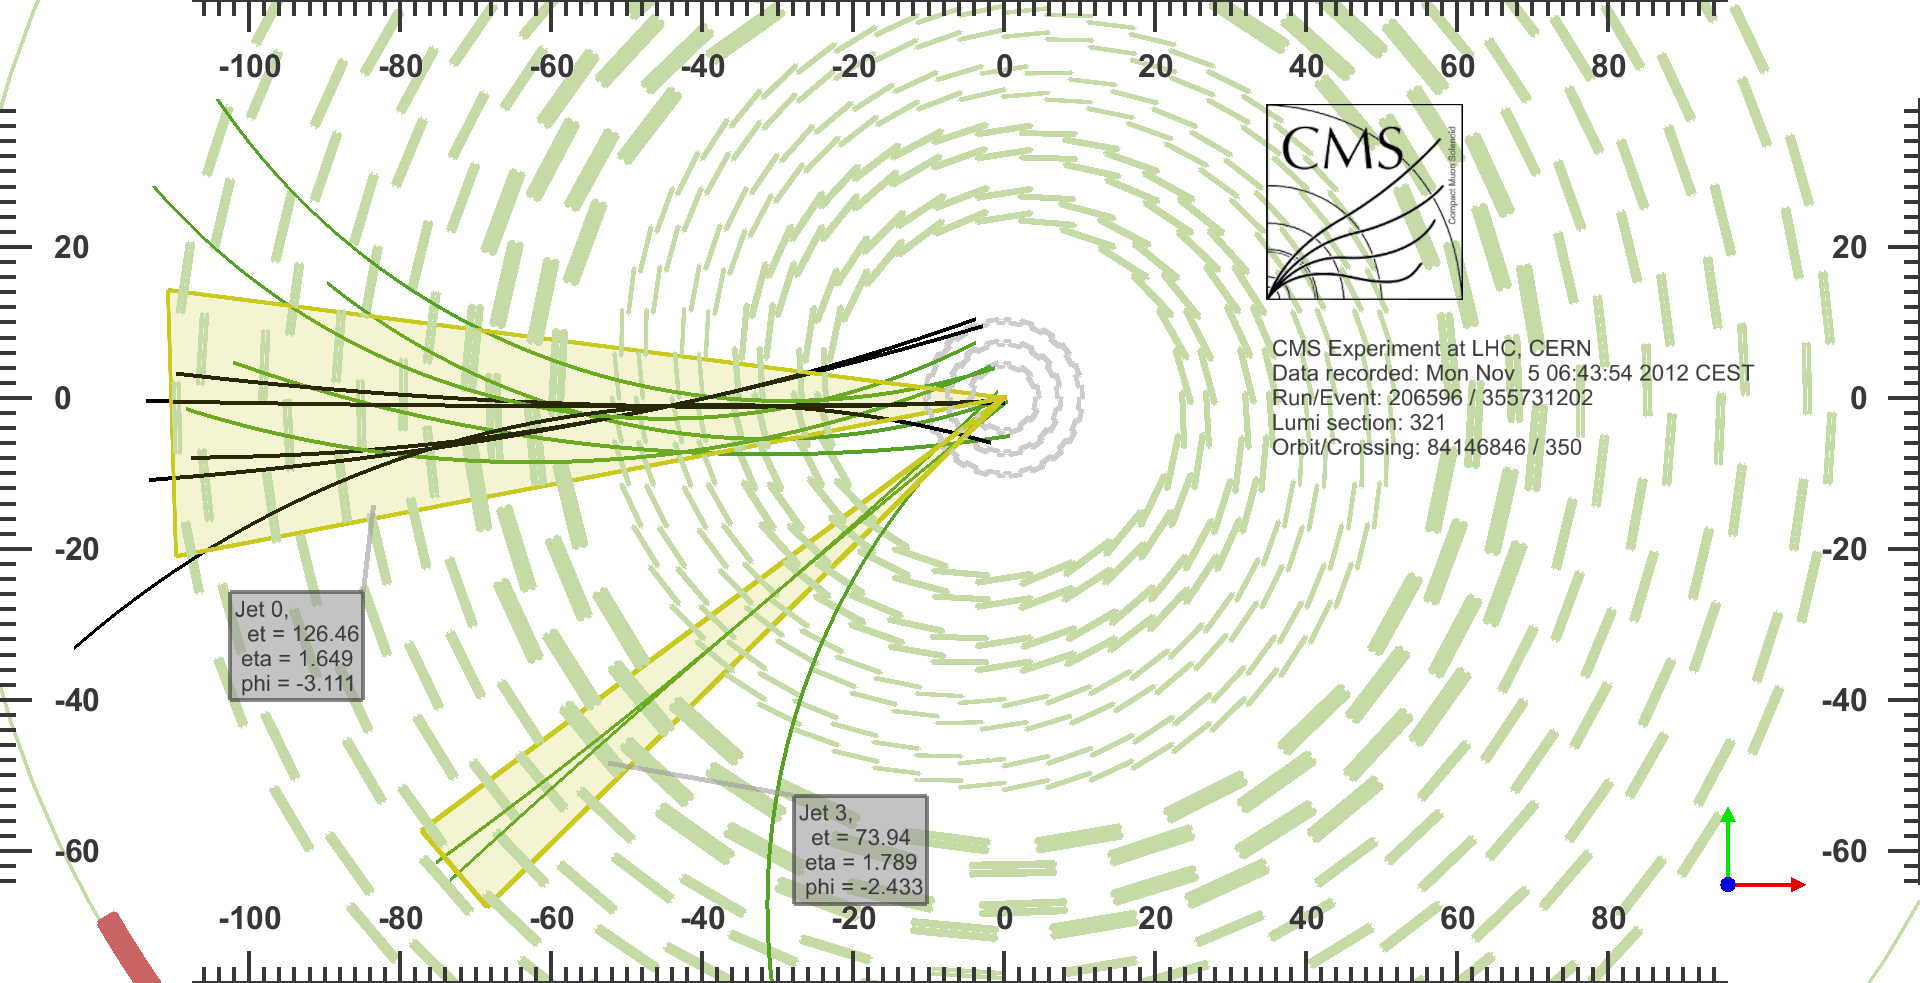
\includegraphics[width=0.9\textwidth]{plots/displays/candidate2_display.png}

\caption{Event displays of the two events passing the optimized selection where only the selected dijet pair
 (yellow cones) and 
the associated tracks (curved lines) are shown, other objects being removed. The tracks that fit the secondary 
vertex are coloured black.  
Candidate 1 (top) with dijet invariant mass of 770 \GeV, which 
passes only the {\it low $L_{xy}$} selection, 
contains a secondary vertex, displaced transversely by 5 \cm, containing 5 tracks from one jet and 1 track
from the other. The 5 track vertex is consistent with a vertex of a B meson with invariant mass below 5 \GeV.
Candidate 2 (bottom) with dijet invariant mass of 75\GeV, 
which passes both {\it low} and {\it high $L_{xy}$} selections, contains a secondary vertex
, displaced transversely by 44 \cm, containing 5 tracks where 2 of these tracks are
associated to both jets due to the jets being nearby. The vertex invariant mass is low and its position
 coincides with one of the silicon 
tracker layers being consistent with a nuclear interaction vertex. \label{fig:eventDisplays}}
\end{figure} 



\section{Limits}
\label{sec:limits}

We set 95\% confidence level
(CL) upper limits for a counting experiment
using the CL$_\mathrm{s}$ method \cite{Read:2002hq, Junk:1999kv}. The limit calculation
takes into account the systematic uncertainties described in Chapter 
\ref{chap:systematics} by introducing
a nuisance parameter for each uncertainty, marginalised by a log-normal prior distribution.

As a first step, upper limits are placed on the mean number of events that could pass
the selection requirements. The resulting observed upper limits are 4.6 events
for the {\it low} $L_{xy}$ selection and 3.7 events for the {\it high} selection.
 These limits are independent
of the particular model assumed for production of long-lived particles given
that the efficiency to pass the selection criteria is not negligible. 


Secondly, an upper limit is quoted on the cross section
to produce $\Higgs \to 2\X$ times the branching fraction squared, $B^2$, for \X to decay into $\qq$.
The observed and
expected limits are shown in Figure \ref{fig:limits}. In order to expand the number of tested models,
the lifetime distributions of the signal MC events are reweighted to
different mean values, namely $0.4\tau$, $0.6\tau$, and $1.4\tau$ for every
lifetime value $\tau$ and mass combination listed
in Table \ref{tab:sigeff}.
Event weights are computed as the product
 of weights assigned to each $\X$ candidate in the event.
The reweighted signal reconstruction efficiencies are then used
to compute the expected and observed limits for these additional mean lifetime values.

\begin{figure}[htbp]
\centering
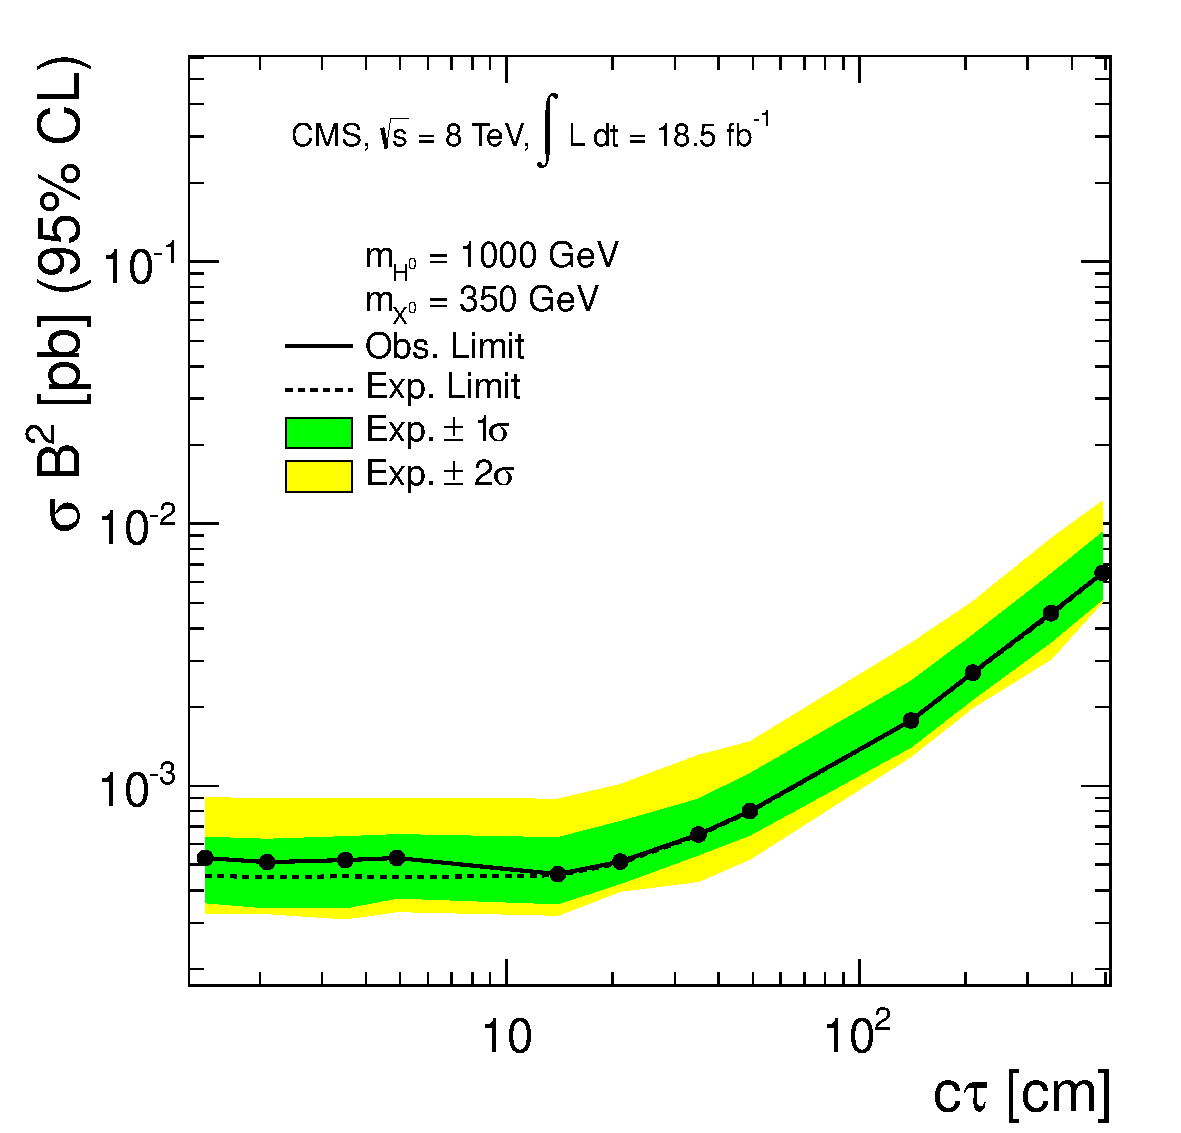
\includegraphics[width=0.49\textwidth]{plots/limits/1000_350e.pdf}
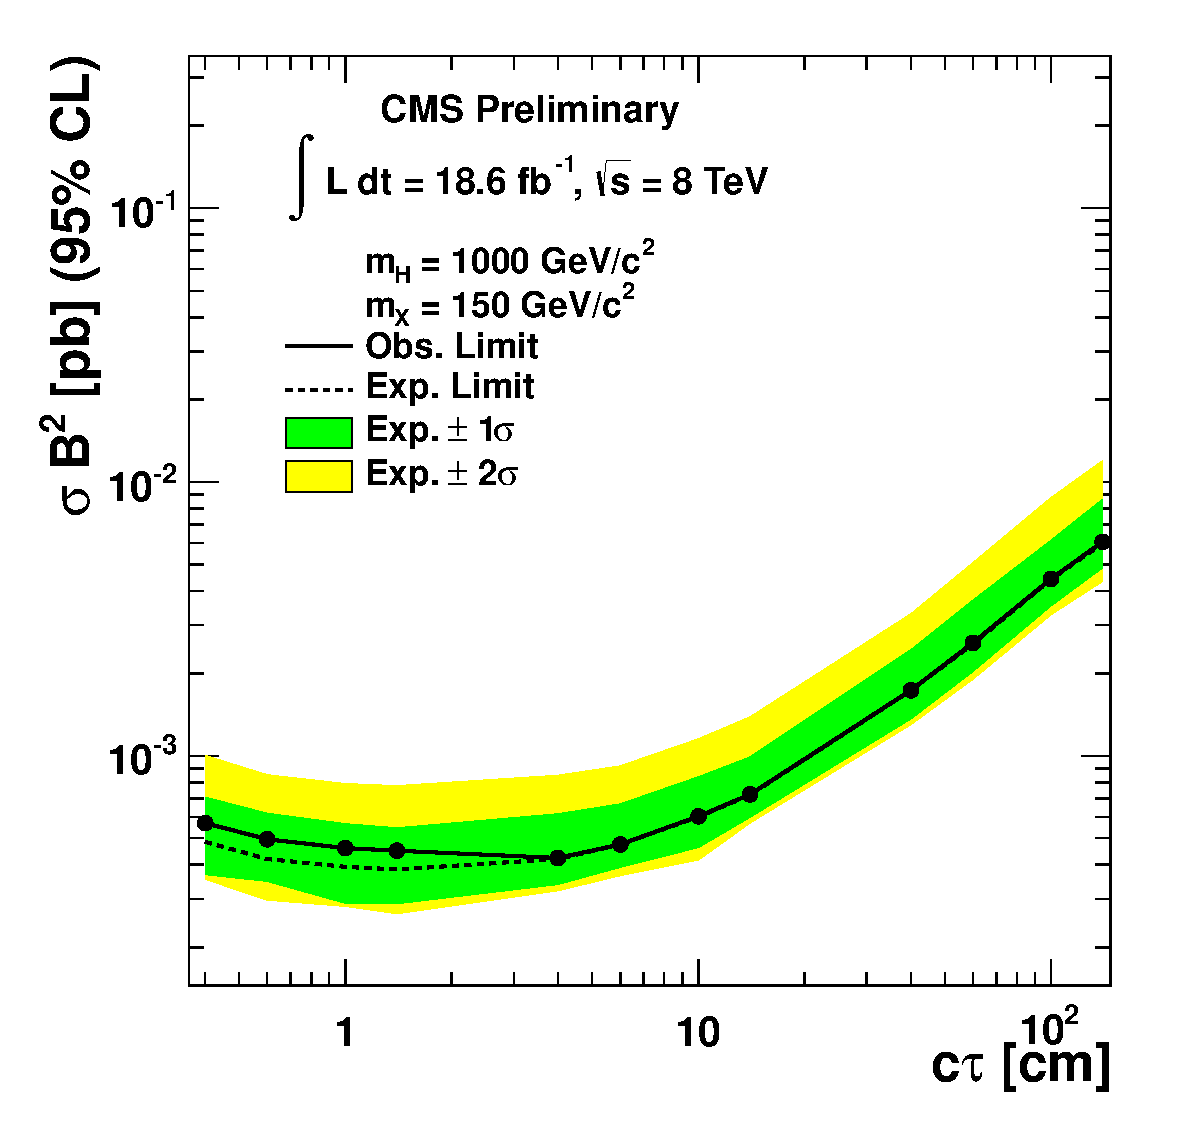
\includegraphics[width=0.49\textwidth]{plots/limits/1000_150e.pdf} 
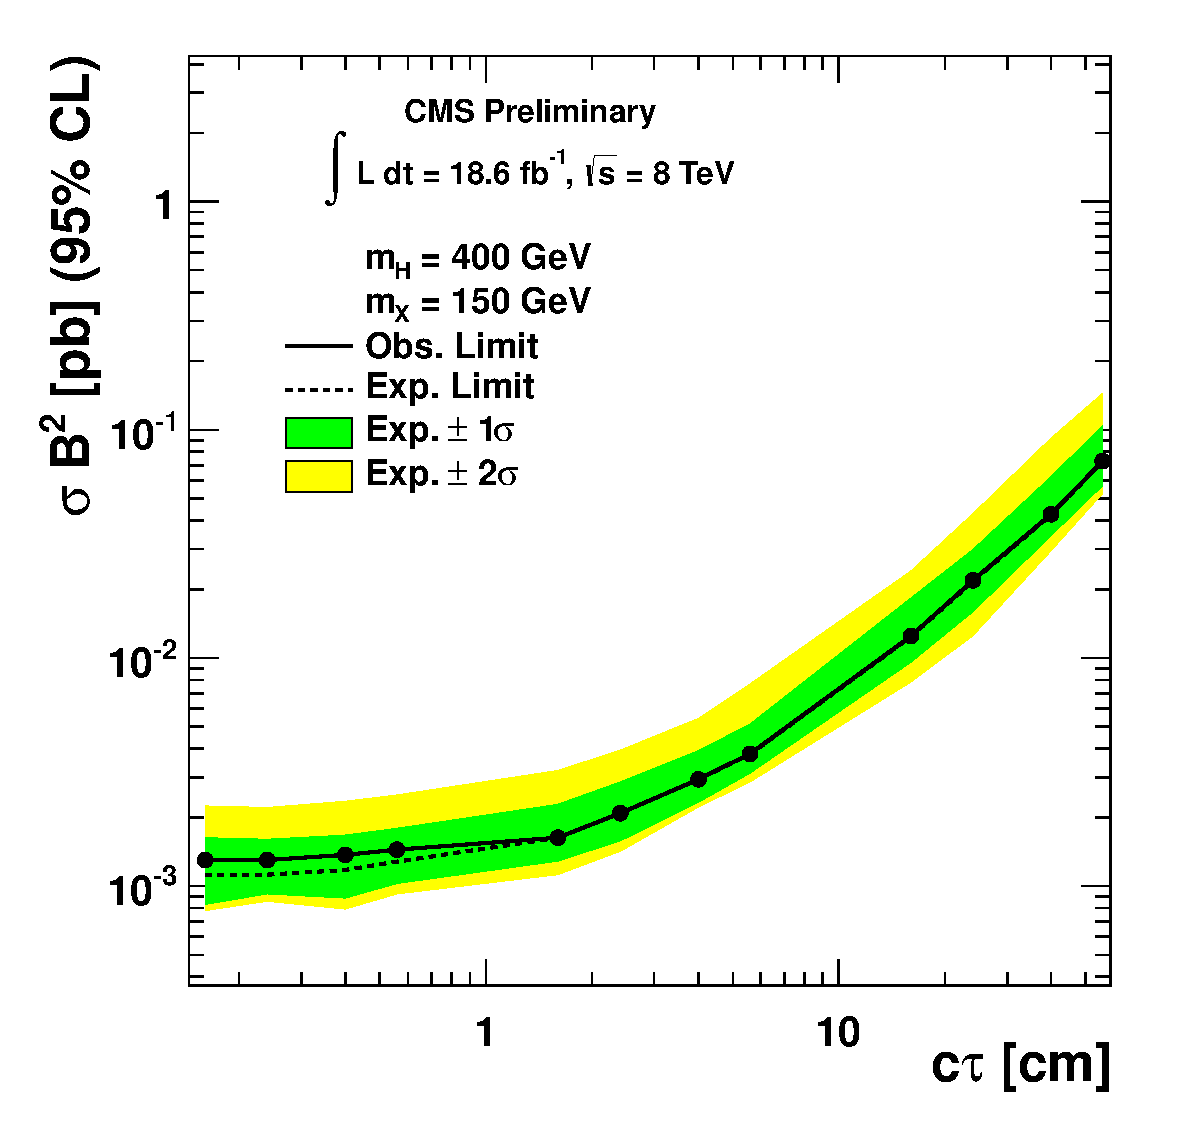
\includegraphics[width=0.49\textwidth]{plots/limits/400_150e.pdf}
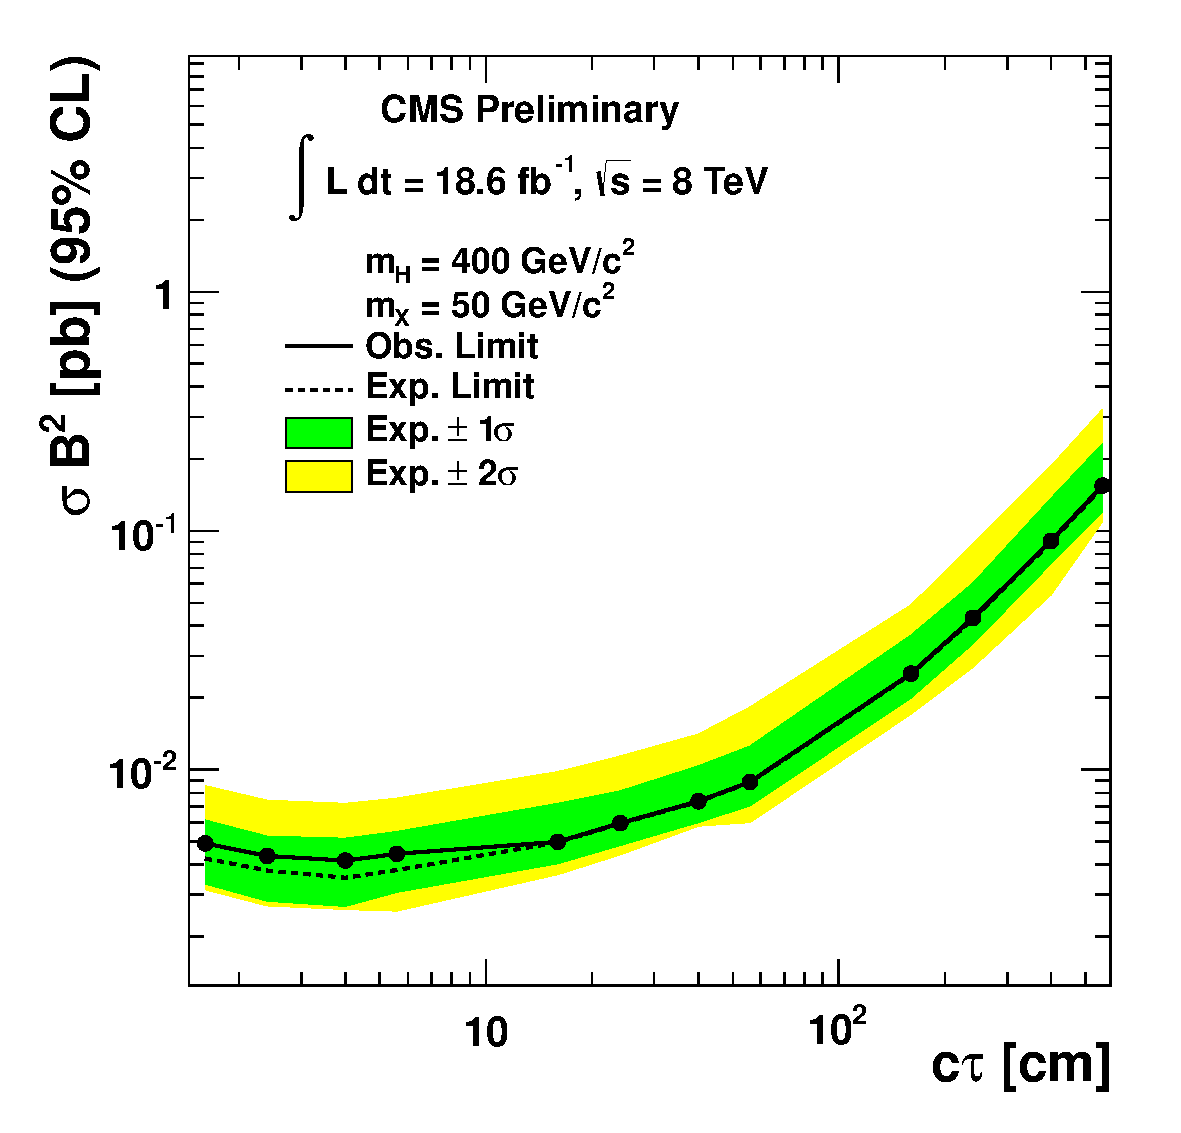
\includegraphics[width=0.49\textwidth]{plots/limits/400_50e.pdf} 
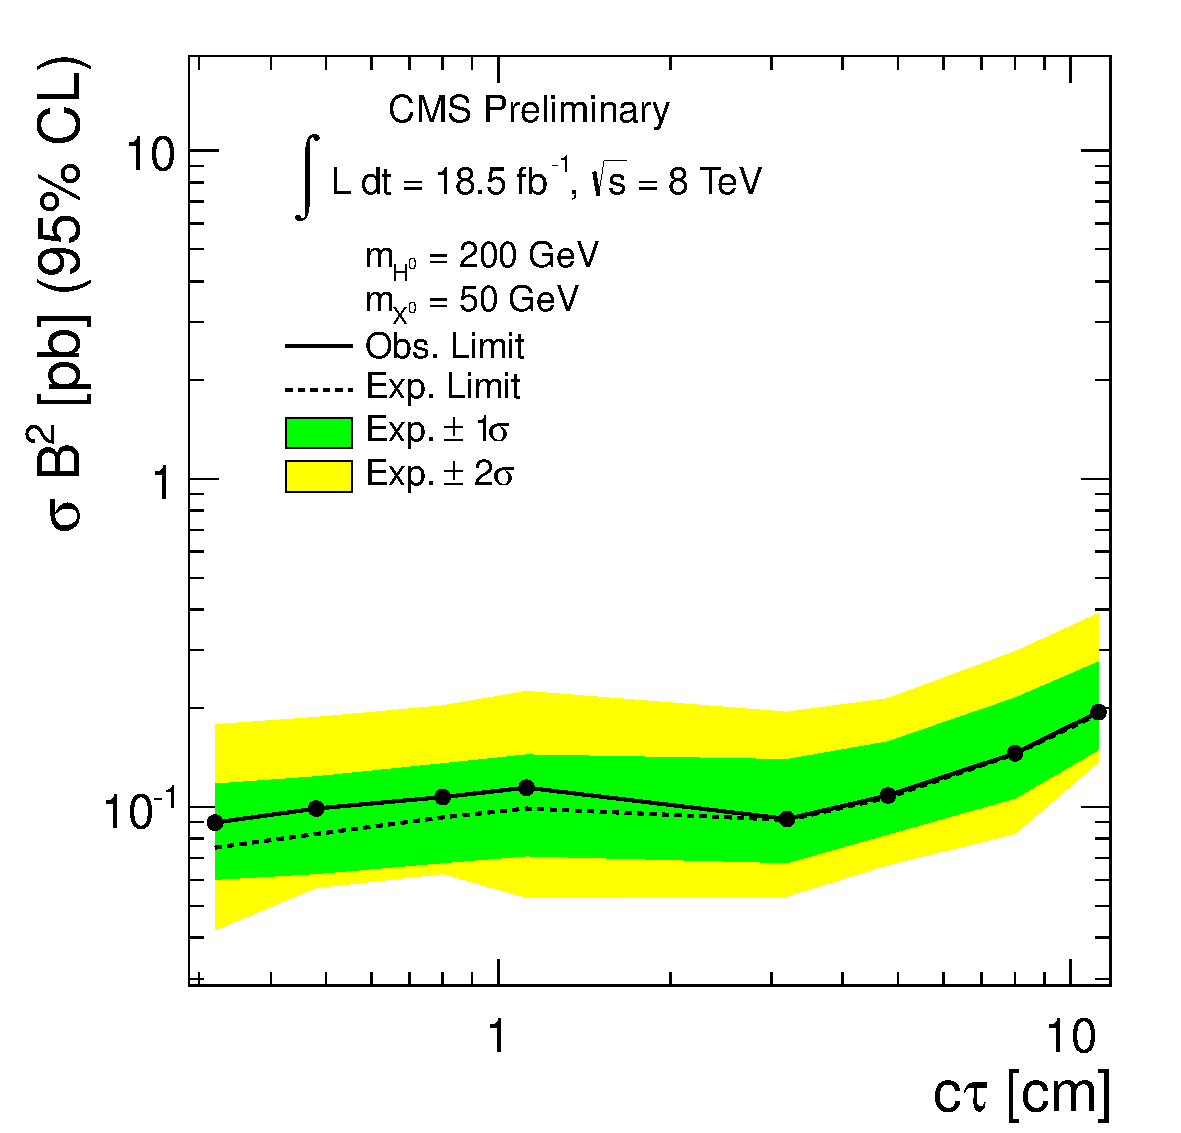
\includegraphics[width=0.49\textwidth]{plots/limits/200_50e.pdf}

\caption{Expected and observed 95\% CL limits for all tested signal models.\label{fig:limits}}
\end{figure}
